\section{Tinjauan Pustaka}

\subsection{EDA (Exploratory Data Analysis)}
% Buat tinjauan pustaka untuk EDA gunakan refrensi yang relevan
Exploratory Data Analysis (EDA) adalah proses analisis data yang bertujuan untuk memahami struktur, pola, dan hubungan dalam dataset sebelum menerapkan model statistik atau machine learning. EDA melibatkan visualisasi data, statistik deskriptif, dan identifikasi anomali atau outlier. Proses ini penting untuk mendapatkan wawasan awal tentang data dan membantu dalam pengambilan keputusan selanjutnya.

\subsection{Regresi Linier}
% Buat tinjauan pustaka untuk regresi linier gunakan refrensi yang relevan
Regresi linier adalah metode statistik yang digunakan untuk memodelkan hubungan antara satu atau lebih variabel independen (fitur) dengan variabel dependen (target). Model ini mengasumsikan bahwa hubungan antara variabel-variabel tersebut dapat direpresentasikan sebagai garis lurus. Regresi linier sering digunakan dalam analisis data untuk prediksi dan inferensi, serta merupakan dasar bagi banyak algoritma machine learning lainnya.

%buat kata kata pengantar untuk bisa membawa rumus regresi linier
Agar dapat memahami bagaimana regresi linier bekerja, kita perlu memahami rumus dasar dari regresi linier. Regresi linier sederhana melibatkan satu variabel independen, sedangkan regresi linier berganda melibatkan beberapa variabel independen. Dalam tugas ini, kita akan fokus pada regresi linier berganda untuk memprediksi jumlah penonton video Youtube berdasarkan metadata yang tersedia.

%masukan rumus regresi linier untuk pemodelan
\begin{equation}
    y = \beta_0 + \beta_1 x_1 + \beta_2 x_2 + ... + \beta_n x_n + \epsilon
\end{equation}

%jelaskan masing masing variabel
Di mana:
\begin{itemize}
    \item $y$ adalah variabel dependen (target).
    \item $\beta_0$ adalah intercept (nilai awal ketika semua variabel independen bernilai nol).
    \item $\beta_1, \beta_2, ..., \beta_n$ adalah koefisien regresi yang menunjukkan pengaruh masing-masing variabel independen terhadap variabel dependen.
    \item $x_1, x_2, ..., x_n$ adalah variabel independen (fitur).
    \item $\epsilon$ adalah error term yang mencakup variasi yang tidak dijelaskan oleh model.
\end{itemize}

%jelaskan kecanggihan teknologi sehingga memudahkan penggunaan regresi linier dalam model machine learning

Dengan kemajuan teknologi dan ketersediaan pustaka machine learning yang kuat seperti scikit-learn, TensorFlow, dan PyTorch, penerapan regresi linier dalam model machine learning menjadi lebih mudah dan efisien. Pustaka-pustaka ini menyediakan fungsi-fungsi yang memungkinkan pengguna untuk dengan cepat membangun, melatih, dan mengevaluasi model regresi linier tanpa harus mengimplementasikan algoritma dari awal.


\subsection{Metadata Youtube}
% Buat tinjauan pustaka untuk metadata Youtube gunakan refrensi yang relevan
Metadata Youtube mencakup berbagai informasi yang terkait dengan video, seperti judul, deskripsi, tag, kategori, dan statistik penonton. Metadata ini sangat penting karena membantu algoritma Youtube dalam merekomendasikan video kepada pengguna dan mempengaruhi visibilitas video di platform. Dengan menganalisis metadata, kita dapat mengidentifikasi faktor-faktor yang berkontribusi terhadap popularitas video dan mengembangkan strategi untuk meningkatkan performa konten.

\begin{figure}[ht]
    \centering
    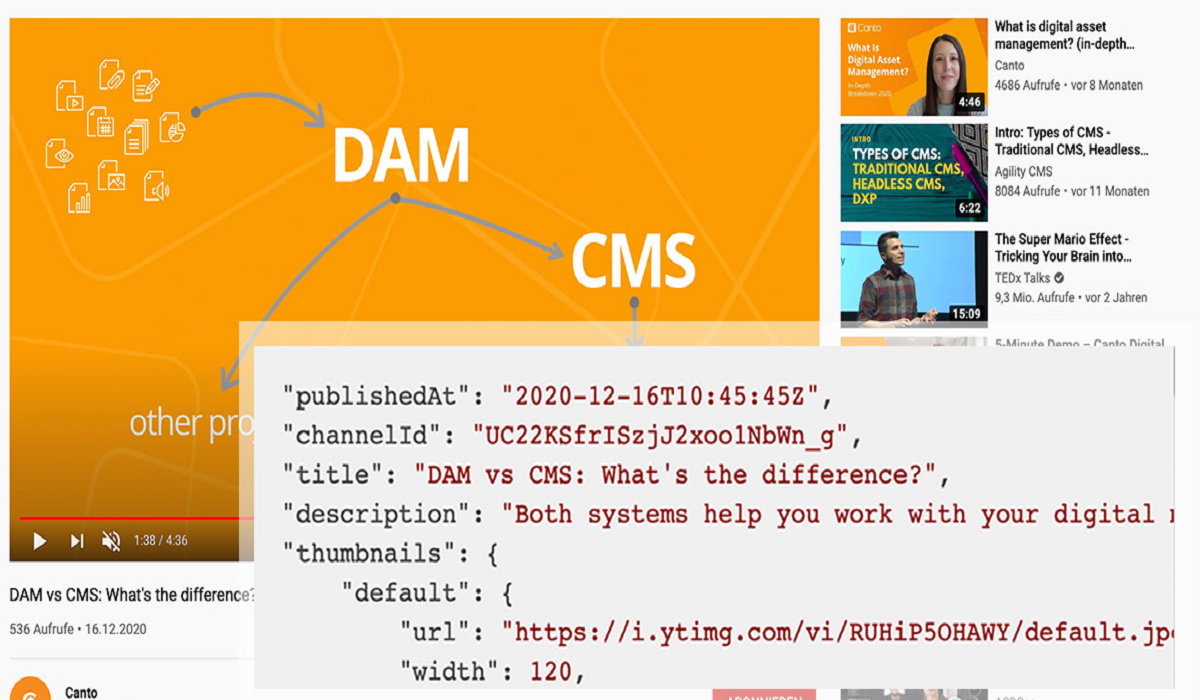
\includegraphics[width=0.8\textwidth]{gambar/youtube-metadata.png}
    \caption{Contoh Metadata Youtube}
    \label{fig:metadata_youtube}
\end{figure}

\subsection{RMSE (Root Mean Square Error)}
% Buat tinjauan pustaka untuk RMSE gunakan refrensi yang relevan
Root Mean Square Error (RMSE) adalah metrik evaluasi yang digunakan untuk mengukur seberapa baik model prediksi dalam memprediksi nilai-nilai numerik. RMSE menghitung akar kuadrat dari rata-rata kuadrat selisih antara nilai yang diprediksi dan nilai aktual. Metrik ini memberikan gambaran tentang seberapa besar kesalahan prediksi model, dengan semakin kecil nilai RMSE menunjukkan performa model yang lebih baik.

\begin{equation}
    RMSE = \sqrt{\frac{1}{n} \sum_{i=1}^{n} (y_i - \hat{y}_i)^2}
\end{equation}

Di mana:
\begin{itemize}
    \item $n$ adalah jumlah data.
    \item $y_i$ adalah nilai aktual.
    \item $\hat{y}_i$ adalah nilai yang diprediksi oleh model.
\end{itemize}

\subsection{$R^2$ (Koefisien Determinasi)}
% Buat tinjauan pustaka untuk $R^2$ gunakan refrensi yang relevan
Koefisien Determinasi ($R^2$) adalah metrik yang digunakan untuk mengukur seberapa baik model regresi menjelaskan variasi dalam data. Nilai $R^2$ berkisar antara 0 hingga 1, di mana nilai yang lebih tinggi menunjukkan bahwa model mampu menjelaskan proporsi yang lebih besar dari variasi dalam data. Metrik ini sering digunakan untuk mengevaluasi performa model regresi dan membandingkan model yang berbeda.

\begin{equation}
    R^2 = 1 - \frac{\sum_{i=1}^{n} (y_i - \hat{y}_i)^2}{\sum_{i=1}^{n} (y_i - \bar{y})^2}
\end{equation}

Di mana:
\begin{itemize}
    \item $n$ adalah jumlah data.
    \item $y_i$ adalah nilai aktual.
    \item $\hat{y}_i$ adalah nilai yang diprediksi oleh model.
    \item $\bar{y}$ adalah rata-rata dari nilai aktual.
\end{itemize}

\subsection{Modeling}
% Buat tinjauan pustaka untuk modeling gunakan refrensi yang relevan
Modeling dalam konteks machine learning adalah proses membangun model matematis atau statistik yang dapat digunakan untuk membuat prediksi atau mengambil keputusan berdasarkan data. Proses ini melibatkan pemilihan algoritma, pelatihan model dengan data, dan evaluasi performa model menggunakan metrik yang relevan. Dalam tugas ini, kita akan fokus pada penerapan regresi linier sebagai metode modeling utama untuk memprediksi jumlah penonton video Youtube berdasarkan metadata yang tersedia.

\subsection{Scikit-learn}
% Buat tinjauan pustaka untuk scikit-learn gunakan refrensi yang relevan
Scikit-learn adalah pustaka machine learning yang populer di Python yang menyediakan berbagai algoritma dan alat untuk analisis data dan modeling. Pustaka ini menawarkan antarmuka yang sederhana dan konsisten, sehingga memudahkan pengguna untuk menerapkan berbagai algoritma machine learning, termasuk regresi linier, klasifikasi, clustering, dan lain-lain. Scikit-learn juga menyediakan fungsi-fungsi untuk preprocessing data, evaluasi model, dan validasi silang, menjadikannya pilihan yang ideal untuk proyek-proyek machine learning.

\subsection{Matplotlib dan Seaborn}

% Buat tinjauan pustaka untuk matplotlib dan seaborn gunakan refrensi yang relevan
Matplotlib dan Seaborn adalah pustaka visualisasi data yang populer di Python. Matplotlib menyediakan fungsi dasar untuk membuat berbagai jenis grafik, seperti garis, batang, dan sebar, sedangkan Seaborn adalah ekstensi dari Matplotlib yang menawarkan antarmuka yang lebih tinggi dan lebih mudah digunakan untuk visualisasi statistik. Keduanya sangat berguna dalam proses EDA (Exploratory Data Analysis) untuk memahami struktur dan pola dalam data melalui visualisasi yang informatif.

\subsection{Pandas}

% Buat tinjauan pustaka untuk pandas gunakan refrensi yang relevan
Pandas adalah pustaka Python yang menyediakan struktur data dan fungsi untuk manipulasi dan analisis data. Pustaka ini menawarkan DataFrame, yang merupakan struktur data tabular yang memungkinkan pengguna untuk dengan mudah mengakses, memanipulasi, dan menganalisis data. Pandas sangat berguna dalam proses EDA (Exploratory Data Analysis) karena menyediakan berbagai fungsi untuk membersihkan, mengolah, dan menganalisis data secara efisien.



\newpage